\documentclass[11pt]{article}


\usepackage[margin=1in,a4paper]{geometry}
\usepackage[utf8]{inputenc}
\usepackage[T1]{fontenc}
\usepackage{lmodern}
\usepackage{tabularx}
\usepackage{quoting}
\usepackage{fancyhdr}
\usepackage{graphicx}
\usepackage{nicefrac}
\usepackage{sectsty}
\usepackage{graphicx}
\usepackage[T1]{fontenc}
\usepackage{epigraph} %quotes
\usepackage{amssymb} %math symbols
\usepackage{mathtools} %more math stuff
\usepackage{amsthm} %theorems, proofs and lemmas
\usepackage{optidef} %fast optimization problem notation
\usepackage{changepage}
\usepackage{gensymb}
\usepackage[ruled,vlined,noend,linesnumbered]{algorithm2e} %algoritms/pseudocode


\usepackage{biblatex}

%% asmthm notation
\newtheorem{theorem}{Theorem}[section]
\newtheorem{corollary}{Corollary}[theorem]
\newtheorem{lemma}[theorem]{Lemma}
\newtheorem{problem}{Problem}
\newtheorem{definition}{Definition}
\newtheorem{claim}{Claim}[section]

\let\oldnl\nl% Store \nl in \oldnl
\newcommand{\nonl}{\renewcommand{\nl}{\let\nl\oldnl}}% Remove line number for one specific line in algorithm

\title{BIOENG-404 - Homework 3: SLIP Models}
\author{
    Nathan Girard
        SV - Neurocomputational
        \and
    Titouan Renard
            MT - Robotics 
}
\date{\today}



\begin{document}


\maketitle

\section{Deliverables}

\begin{enumerate}
    \item Plot a graph with several successful solutions as the ones shown in Figure 2 of Seyfarth et al.
    \begin{adjustwidth}{0.5cm}{}
        \begin{figure}[h!]
            \centering
            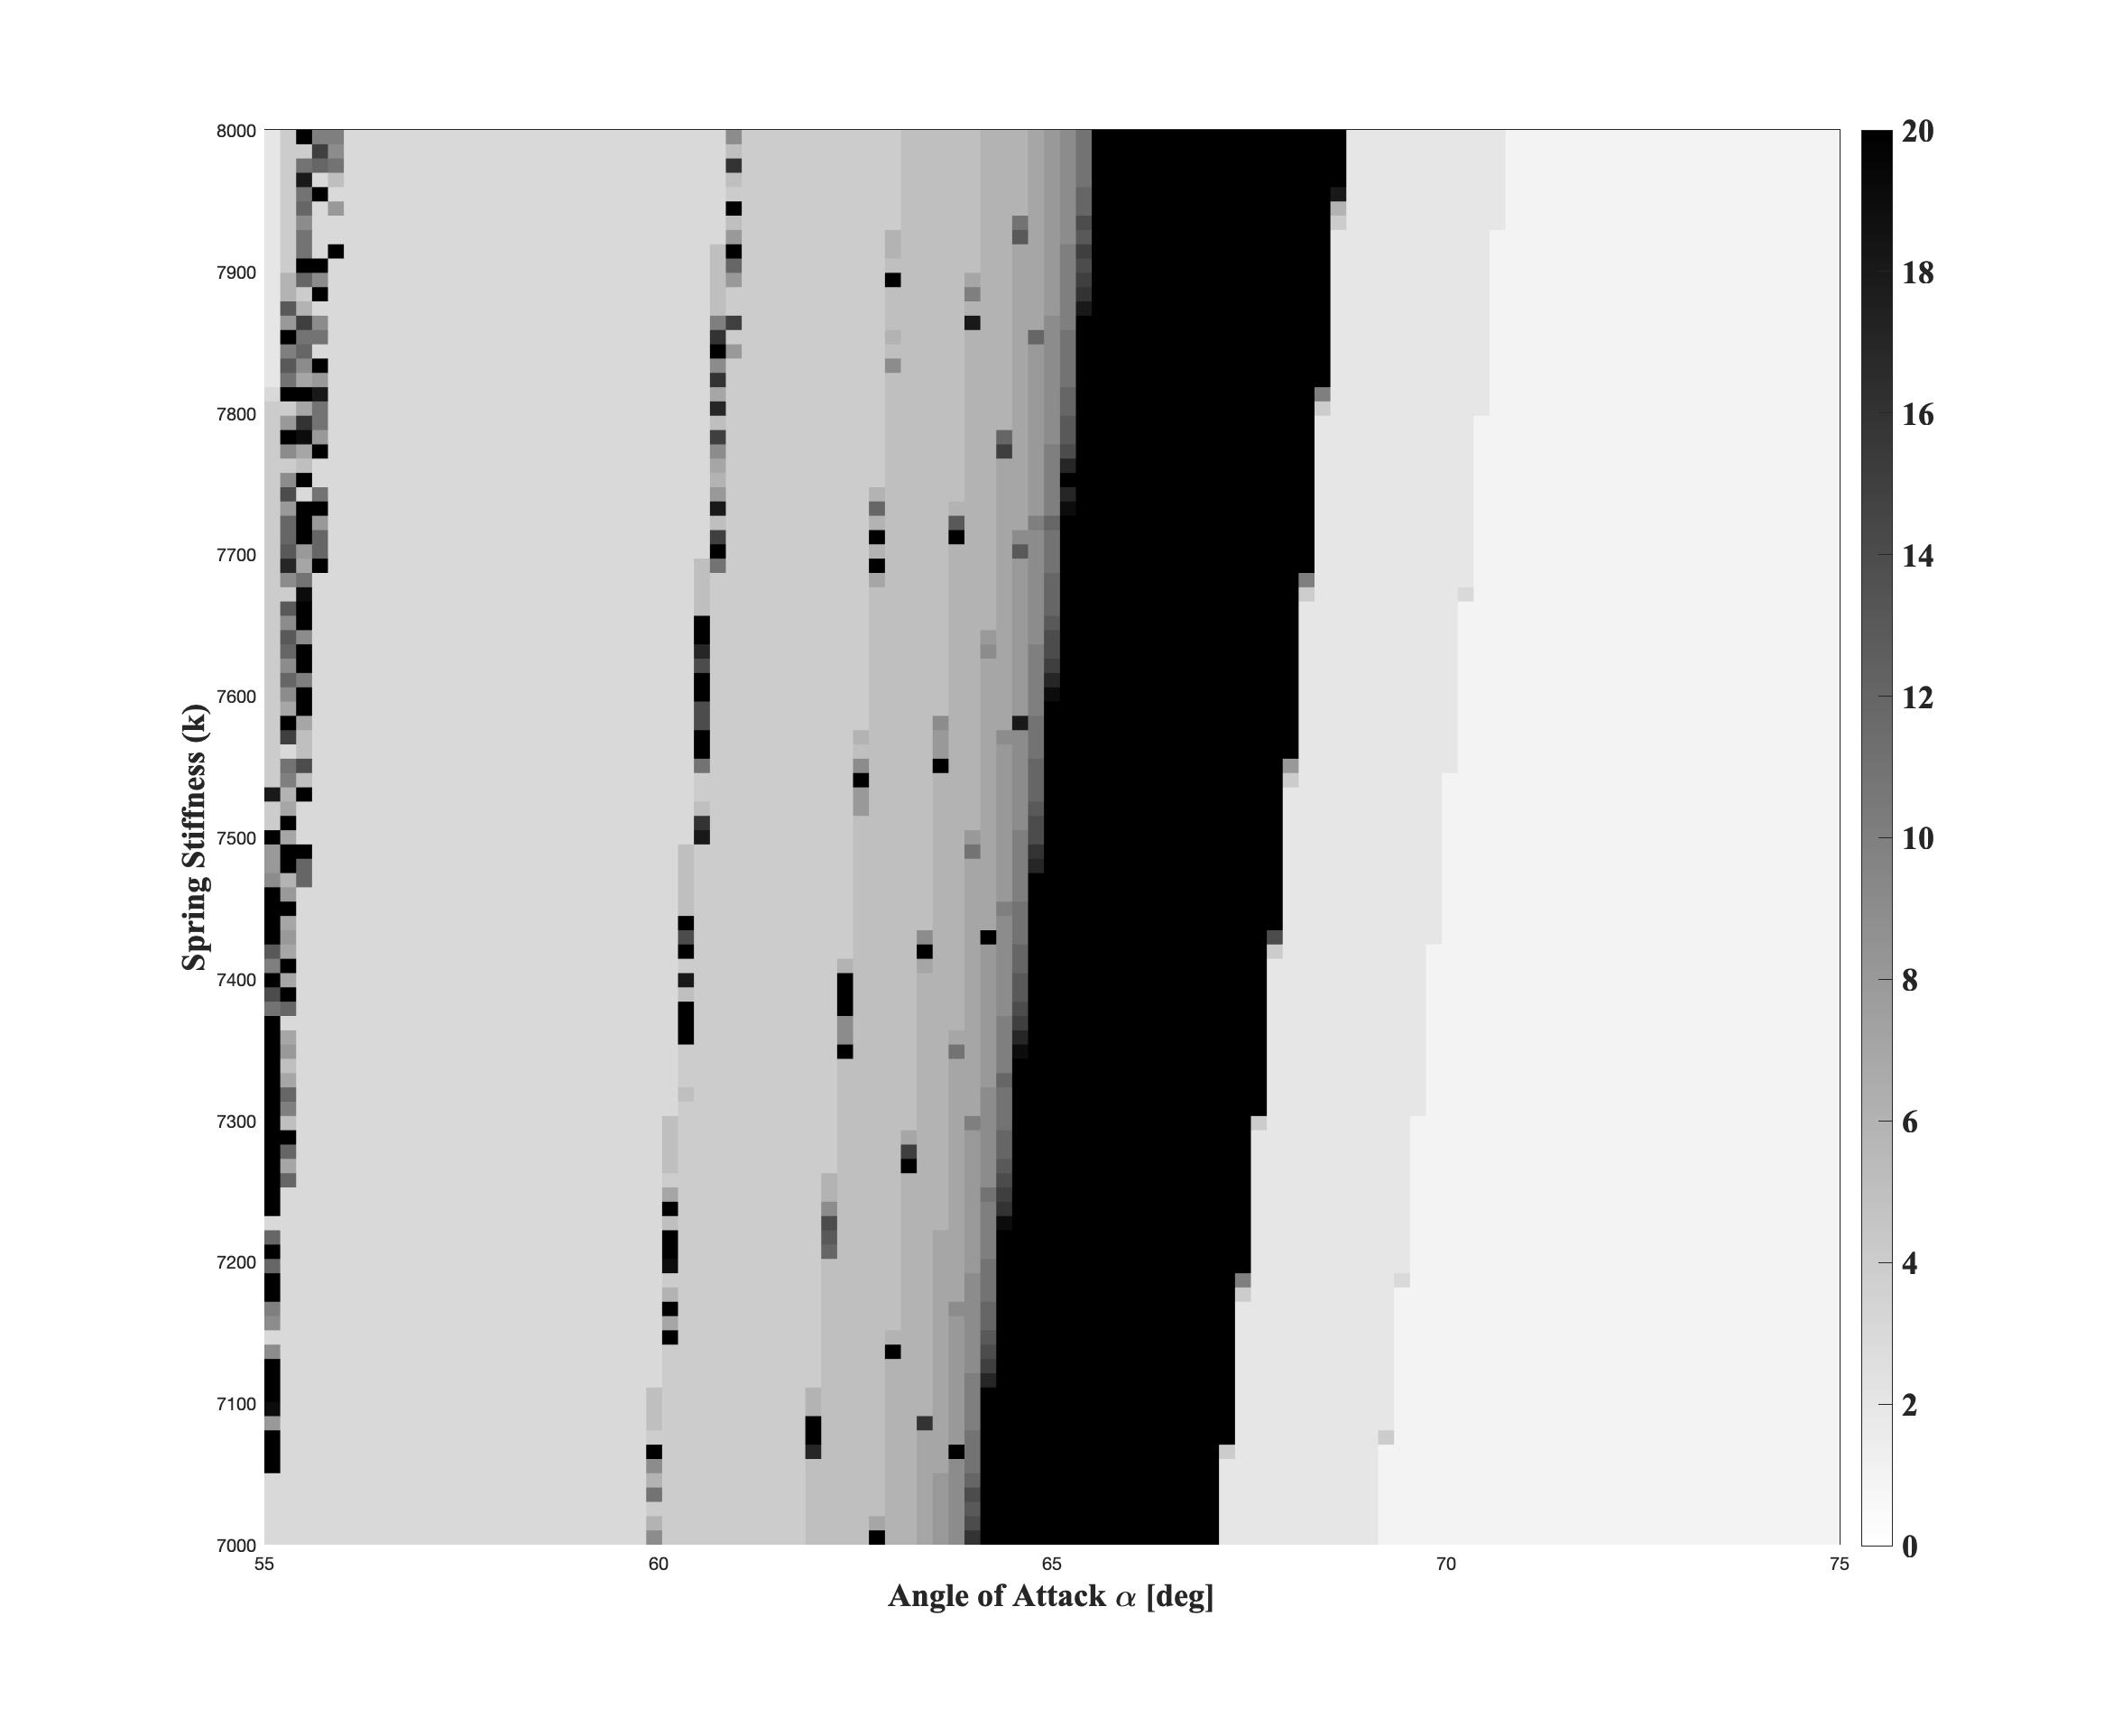
\includegraphics[width=0.9\textwidth]{screens/plot_2.jpg}
            \caption{Stability (measured in step numbers) for different $K$ (spring stiffness) and $\alpha$ (angle of attack) values.}
            \label{stability_domain}
        \end{figure}
    \end{adjustwidth}

    \item Explain the trend you observe in the graph and its meaning from a biomechanics perspective.
    \begin{adjustwidth}{0.5cm}{}
        From the graph, we observe that the running gait is only stable on a limited domain of initial conditions (here we observe the evolution of stability as a function of spring stiffness $K$ and angle of attack $\alpha$, while using fixed) : the so called \textit{running domain}. On the graph we observe that the domain for which the model produces stable running are placed along a "J" shaped line with equation 
        \[ K \cdot (1 - \sin \alpha) = \text{const}. \]
        This result closely matches experimental data for leg-stiffness to angle of attack in human running as has been shown by Seyfarth et al. \cite{1}. This suggests that a simple model such as SLIP accurately captures the fundamental dynamics of running in biology.
    \end{adjustwidth}

    \item Do you think counting the number of steps is a good measure of stability? How can a Return Map (or Poincaré Map) be used to evaluate the system's stability? For more details on this method, please refer to the lecture notes as well as the reference.
    \begin{adjustwidth}{0.5cm}{}
        Step number provides 
    \end{adjustwidth}

    \item Which aspects of human locomotion's biomechanics can be investigated with this type of model, ad which one cannot be investigated?Which aspects of human locomotion's biomechanics can be investigated with this type of model, ad which one cannot be investigated?
    \begin{adjustwidth}{0.5cm}{}
        
    \end{adjustwidth}
\end{enumerate}

\begin{figure}[h!]
    \centering
    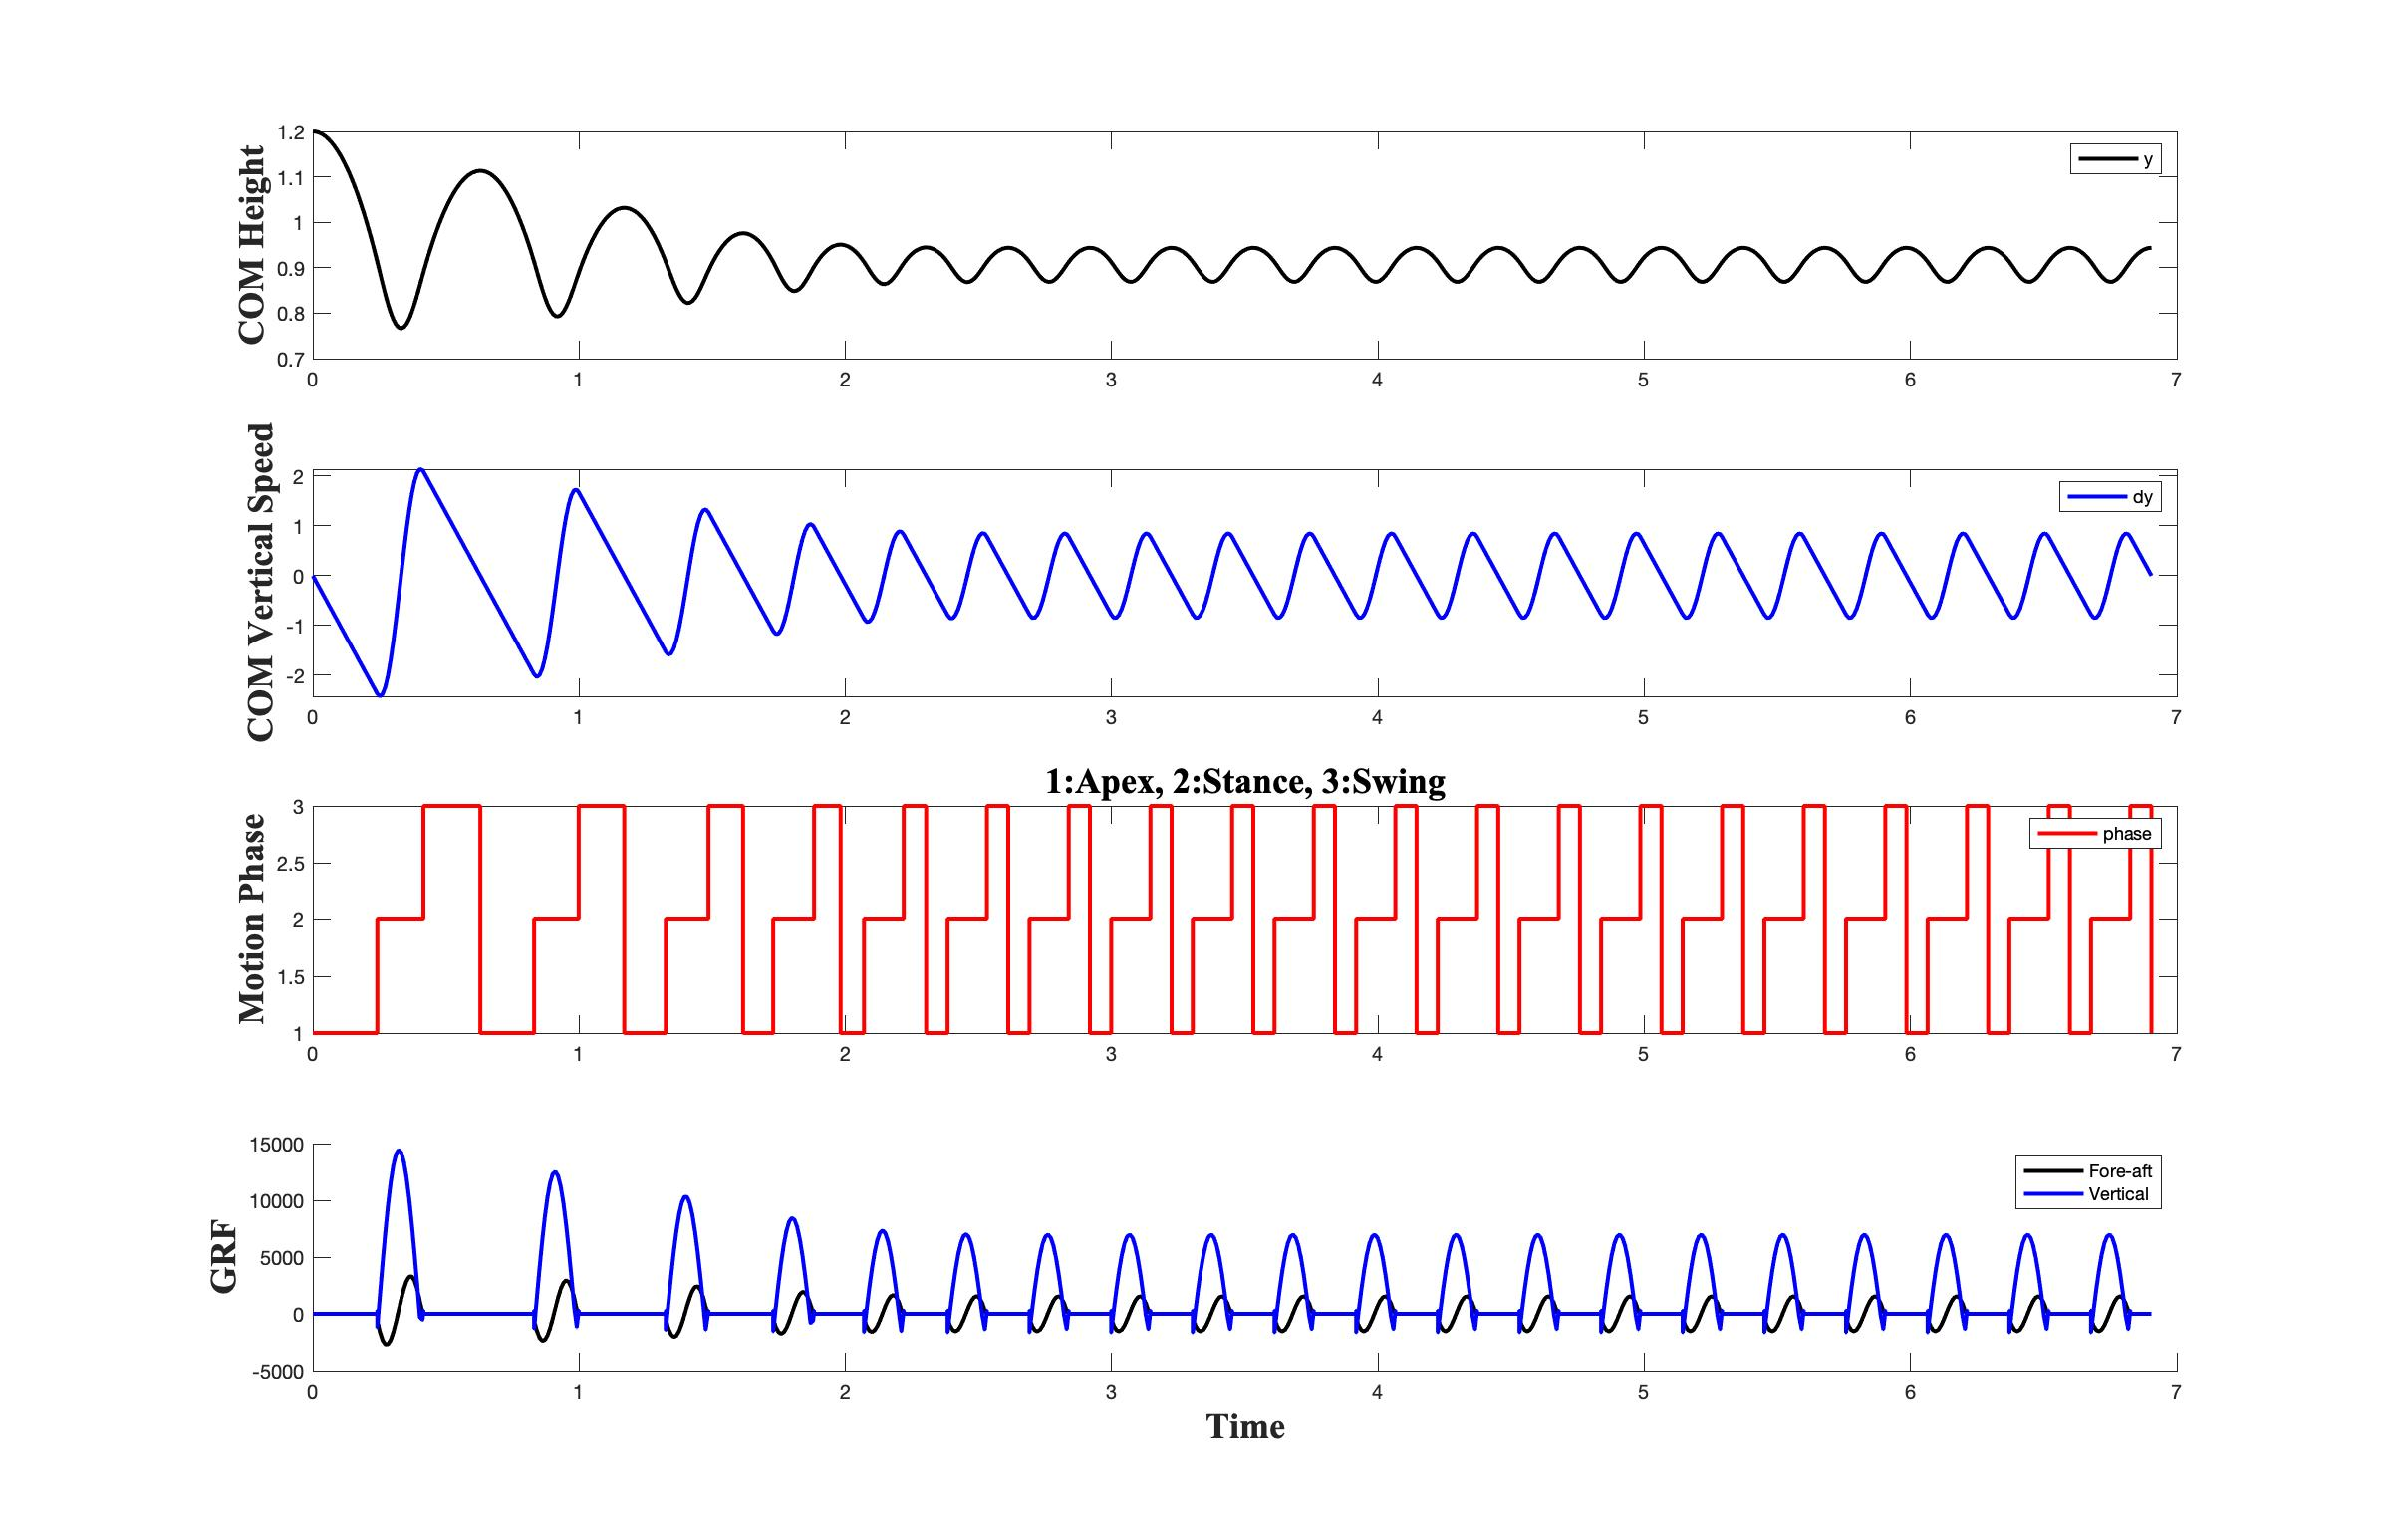
\includegraphics[width=0.9\textwidth]{screens/run_1.jpg}
    \caption{trajectories of a stable (over $20$ steps) solution for the SLIP.}
\end{figure}

\begin{thebibliography}{1}

    \bibitem{SeyfarthBiomecha} Andre Seyfarth, Hartmut Geyera, Michael Gunther, Reinhard Blickhan, "\textit{A movement criterion for running}" \emph{Journal of Biomechanicsn 35}, pp. 649-655, 2001.

\end{thebibliography}


\end{document}

